\documentclass[oneside,10pt]{book}
\usepackage{graphicx}
\graphicspath{{pictures/}}% Specifies where pictures are stored
\usepackage{docmute} % for muting preamble of input files
\usepackage[top=0.65in,bottom=0.50in,left=0.75in,right=0.75in]{geometry}
\usepackage{amsmath}
\usepackage{amssymb}
\usepackage{multicol}
\usepackage{booktabs}
\usepackage[shortlabels]{enumitem}

\usepackage[activate={true,nocompatibility},final,tracking=true,kerning=true,spacing=true,factor=1100,stretch=10,shrink=10]{microtype}

\usepackage{subcaption} % for \captionof command
\usepackage{mathpazo} % Times
\usepackage[T1]{fontenc}
\usepackage[semibold]{raleway}

\usepackage[usenames,dvipsnames,svgnames]{xcolor} % for colors
\definecolor{ocre}{RGB}{0,135,255} % main color
\definecolor{maincolor}{RGB}{0,145,255} % main color
\definecolor{cqcqcq}{rgb}{0.75294117,0.75294117647,0.75294117647}

\usepackage{tikz}
\usetikzlibrary{arrows.meta, arrows}

\usepackage{xargs}
\usepackage{colortbl} % for colored tables
\usepackage{hyperref}
%\hypersetup{
    %colorlinks=true,
    %linkcolor=blue,
    %filecolor=magenta,
    %urlcolor=cyan,
%}





\makeatletter
%%%%%%%%%%%%%%%%%%%%%%%%%%%%%%%%%%%%%%%%%%%%%%%%%%%%%%%%%%%%%%%%%%%
% Set indent to zero, but save value just in case
%%%%%%%%%%%%%%%%%%%%%%%%%%%%%%%%%%%%%%%%%%%%%%%%%%%%%%%%%%%%%%%%%%%
\newlength\tindent
\setlength{\tindent}{\parindent}
\setlength{\parindent}{0pt}
\renewcommand{\indent}{\hspace*{\tindent}}
%%%%%%%%%%%%%%%%%%%%%%%%%%%%%%%%%%%%%%%%%%%%%%%%%%%%%%%%%%%%%%%%%%%
%%%%%%%%%%%%%%%%%%%%%%%%%%%%%%%%%%%%%%%%%%%%%%%%%%%%%%%%%%%%%%%%%%%

\newcounter{ExampleCounter}[section]
\newcommand{\example}{%
  \vspace{4pt minus 3pt}
  \par%
  \refstepcounter{ExampleCounter}%
  \noindent\textbf{Example~\arabic{ExampleCounter}.\,~}%
}



%%%%%%%%%%%%%%%%%%%%%%%%%%%%%%%%%%%%%%%%%%%%%%%%%%%%%%%%%%%%%%%%%%%
% grid command
%%%%%%%%%%%%%%%%%%%%%%%%%%%%%%%%%%%%%%%%%%%%%%%%%%%%%%%%%%%%%%%%%%%
\newcommand{\grid}[1]{%
\begin{tikzpicture}
  \draw[step=.5cm,cqcqcq,very thin] (-#1/2,-#1/2) grid (#1/2,#1/2);
\end{tikzpicture}
}


\newcommandx{\cart}[3][2=1,3={}]{%
\par
\begin{tikzpicture}[scale=#2]
  \draw[step=.5cm,cqcqcq,very thin] (-#1/2,-#1/2) grid (#1/2,#1/2);
  \draw[<->, black] (-#1/2,0) -- (#1/2,0);
  \draw[<->, black] (0, -#1/2) -- (0, #1/2);
  #3
\end{tikzpicture}
\par
}


\newcommandx{\cartX}[6][5=1,6={}]{%
\par
\begin{tikzpicture}[scale=#5]
  \draw[step=1cm,cqcqcq,very thin] (#1,#3) grid (#2,#4);
  \draw[<->, black] (#1,0) -- (#2,0);
  \draw[<->, black] (0, #3) -- (0, #4);
  #6
\end{tikzpicture}
\par
}
%%%%%%%%%%%%%%%%%%%%%%%%%%%%%%%%%%%%%%%%%%%%%%%%%%%%%%%%%%%%%%%%%%%
%%%%%%%%%%%%%%%%%%%%%%%%%%%%%%%%%%%%%%%%%%%%%%%%%%%%%%%%%%%%%%%%%%%


%%%%%%%%%%%%%%%%%%%%%%%%%%%%%%%%%%%%%%%%%%%%%%%%%%%%%%%%%%%%%%%%%%%%%%%%%%%
% Headings
%%%%%%%%%%%%%%%%%%%%%%%%%%%%%%%%%%%%%%%%%%%%%%%%%%%%%%%%%%%%%%%%%%%%%%%%%%%


\usepackage{titlesec}

\titleformat{\chapter}[display]
  {\sffamily\huge\bfseries}{\color{maincolor}
  {\chaptertitlename\ \thechapter}}{0pt}{\Huge}[]
\titleformat{\section}
  {\sffamily\LARGE\bfseries}
  {\color{maincolor}{\thesection}}{8pt}{}[]
\titleformat{\subsection}
  {\sffamily\Large\bfseries}{}{0ex}{}
\titleformat{\subsubsection}
  {\sffamily\normalsize\bfseries}{\thesubsubsection}{1ex}{}
\titleformat{\paragraph}[runin]
  {\sffamily\normalsize\bfseries}{\theparagraph}{1em}{}
\titleformat{\subparagraph}
  {\sffamily\LARGE\bfseries}
  {\color{maincolor}{\thesection}}{8pt}{}[]

\titlespacing*{\chapter} {0in}{0pt}{9pt}
\titlespacing*{\section} {0in}{3.5ex plus 1ex minus .2ex}{3.3ex plus .2ex}
\titlespacing*{\subsection} {0pt}{3.25ex plus 1ex minus .2ex}{1.5ex plus .2ex}
\titlespacing*{\subsubsection}{0pt}{3.25ex plus 1ex minus .2ex}{0.5ex plus .2ex}
\titlespacing*{\paragraph} {0pt}{3.25ex plus 1ex minus .2ex}{1em}
%\titlespacing*{\subparagraph} {\parindent}{3.25ex plus 1ex minus .2ex}{1em}
\titlespacing*{\subparagraph} {-0in}{3.5ex plus 1ex minus .2ex}{2.3ex plus .2ex}

\renewcommand{\bottomtitlespace}{2.5in}
%\newcommand{\sectionbreak}{\clearpage}
%\newcommand{\chapterbreak}{\cleardoublepage}


%%%%%%%%%%%%%%%%%%%%%%%%%%%%%%%%%%%%%%%%%%%%%%%%%%%%%%%%%%%%%%%%%%%%%%
%%%%%%%%%%%%%%%%%%%%%%%%%%%%%%%%%%%%%%%%%%%%%%%%%%%%%%%%%%%%%%%%%%%%%%

\newcommand{\setsection}[2]{%
  \setcounter{chapter}{#1}
  \setcounter{section}{#2}
  \addtocounter{section}{-1}

}

%%%%%%%%%%%%%%%%%%%%%%%%%%%%%%%%%%%%%%%%%%%%%%%%%%%%%%%%%%%%%%%%%%%%%%%%%%%
% Table of Contents Styling
%%%%%%%%%%%%%%%%%%%%%%%%%%%%%%%%%%%%%%%%%%%%%%%%%%%%%%%%%%%%%%%%%%%%%%%%%%%


\usepackage{titletoc} % Required for manipulating the table of contents
\contentsmargin{0cm} % Removes the default margin


% Part text styling
\titlecontents{part}[0cm]
{\addvspace{20pt}\centering\large\bfseries}
{}
{}
{}

% Chapter text styling
\titlecontents{chapter}[1.00cm] % Indentation
{\addvspace{5pt}\Large\sffamily\bfseries} % Spacing and font options for chapters
{\color{maincolor}\contentslabel[\Large\thecontentslabel]{1.00cm}\color{maincolor}} % Chapter number
{\color{maincolor}}
{\color{maincolor}\Large\;\titlerule*[.5pc]{.}\;\thecontentspage} % Page number

% Section text styling
\titlecontents{section}[1.75em] % Indentation
{\addvspace{5pt}\large\sffamily\bfseries} % Spacing and font options for chapters
{\color{maincolor}\contentslabel[\large\thecontentslabel]{1.75em}\color{black}} % Chapter number
{\color{black}}
{\color{black}\large\;\titlerule*[.5pc]{.}\;\thecontentspage} % Page number
[]

% Subsection text styling
\titlecontents{subsection}[1.75em] % Indentation
{\addvspace{0pt}\sffamily\small} % Spacing and font options for subsections
{} % Subsection number
{}
{\ \titlerule*[.5pc]{.}\;\thecontentspage} % Page number
[]


%%%%%%%%%%%%%%%%%%%%%%%%%%%%%%%%%%%%%%%%%%%%%%%%%%%%%%%%%%%%%%%%%%%%%%%%%%%
% PAGE HEADERS
%%%%%%%%%%%%%%%%%%%%%%%%%%%%%%%%%%%%%%%%%%%%%%%%%%%%%%%%%%%%%%%%%%%%%%%%%%%


\usepackage{ifthen}
\usepackage{fancyhdr} % Required for header and footer configuration

\pagestyle{fancy}

\renewcommand{\chaptermark}[1]{\markboth{\normalsize\bfseries\chaptername\ \thechapter\ \ #1}{}} % Chapter text font settings

\renewcommand{\sectionmark}[1]{\markright{\normalsize\thesection\hspace{5pt}#1}{}} % Section text font settings
\fancyhf{}


\fancyhead[R]{\sffamily\rightmark\hspace{5ex}\thepage}
%\fancyhead[L]{\ifthenelse{\isodd{\value{page}}}{}{\sffamily\thepage\hspace{5ex} \leftmark}}


\renewcommand{\headrulewidth}{0pt}
\renewcommand{\footrulewidth}{0pt} % Removes the rule in the footer

\addtolength{\headheight}{2.5pt} % Increase the spacing around the header slightly

%%%%%%%%%%%%%%%%%%%%%%%%%%%%%%%%%%%%%%%%%%%%%%%%%%%%%
%%%%%%%%%%%%%%%%%%%%%%%%%%%%%%%%%%%%%%%%%%%%%%%%%%%%%
% define a command to insert a blank page
        \newcommand{\insertblankpage}{%
          \newpage
          \thispagestyle{empty}
          \mbox{}
        \addtocounter{page}{-1}
          \newpage
        }
%%%%%%%%%%%%%%%%%%%%%%%%%%%%%%%%%%%%%%%%%%%%%%%%%%%%%
%%%%%%%%%%%%%%%%%%%%%%%%%%%%%%%%%%%%%%%%%%%%%%%%%%%%%



%%%%%%%%%%%%%%%%%%%%%%%%%%%%%%%%%%%%%%%%%%%%%%%%%%%%%
% Define Objectives Environment
%%%%%%%%%%%%%%%%%%%%%%%%%%%%%%%%%%%%%%%%%%%%%%%%%%%%%
\usepackage{environ}

\NewEnviron{objectives}[1]{%
\vspace{0.5em}
\noindent\textbf{\sffamily\Large Objectives}

\vspace{2mm}

\noindent%
#1

\vspace{-2.5mm}
\begin{multicols}{2}
\begin{itemize}[nosep,leftmargin=10.0pt]
    \BODY
\end{itemize}
\end{multicols}

}


%%%%%%%%%%%%%%%%%%%%%%%%%%%%%%%%%%%%%%%%%%%%%%%%%%%%%%%%%%%%%%%%%%%
% Create blue box for definitions and theorems
%%%%%%%%%%%%%%%%%%%%%%%%%%%%%%%%%%%%%%%%%%%%%%%%%%%%%%%%%%%%%%%%%%%


\tikzstyle{bluebox} = [fill=ocre!10, draw=ocre, very thick,
    rectangle, rounded corners, inner sep=10pt, inner ysep=5pt]
\tikzstyle{fancytitle} =[fill=ocre, text=white, rounded corners,
    inner ysep=3pt, inner xsep=5pt]



\def\blueboxstring{bluebox}


\newcommand{\bluebox}[2]{%
\par
\vspace{2mm minus 1mm}
\begin{tikzpicture}%
\node [bluebox] (box){%
    \begin{minipage}{0.99\textwidth}%
      \vspace{7pt}
      #2
    \end{minipage}
};
\node[fancytitle, right=10pt] at (box.north west) {%
  #1
};
\end{tikzpicture}
\par
\vspace{2mm}
}


%\NewEnviron{bluebox}[1]{%
%\par
%\vspace{2mm minus 1mm}
%\begin{tikzpicture}%
%\node [bluebox] (box){%
    %\begin{minipage}{0.99\textwidth}%
      %\vspace{7pt}
      %\expandafter\BODY
    %\end{minipage}
%};
%\node[fancytitle, right=10pt] at (box.north west) {%
  %#1
%};
%\end{tikzpicture}
%\par
%\vspace{2mm}
%}


%\let\blueboxenvironment\bluebox


%\def\bluebox#1{%
  %\ifx\@currenvir\blueboxstring%
    %\blueboxenvironment
  %\else
    %\blueboxcommand
  %\fi
%}



%%%%%%%%%%%%%%%%%%%%%%%%%%%%%%%%%%%%%%%%%%%%%%%%%%%%%
% Redefine vfill command to take optional parameter
%%%%%%%%%%%%%%%%%%%%%%%%%%%%%%%%%%%%%%%%%%%%%%%%%%%%%

\renewcommand{\vfill}[1][1]{\vspace{\stretch{#1}}}

\makeatother


\usepackage{multicol}
\usepackage{array}
\usepackage{booktabs}
\usepackage{subcaption}



\title{Lecture Notes}
\graphicspath{{3-4-lecture/}}

\AtBeginDocument{%
  \large
}

\begin{document}

\setcounter{chapter}{3}
\setcounter{section}{3}

\section{Library of Functions and Piecewise Functions}


\textit{Sometimes the questions are complicated and the answers are simple.}
--Dr.~Suess


\begin{objectives}
{In this section we will}
  \item
    graph the library of functions.
  \item
    learn to graph piecewise functions.
  \item
    learn to construct piecewise functions.
  \item
    identify the $x$-intercept and $y$-intercept of a graph.
\end{objectives}



%TODO
%\example
%Graph
%\cart{7}
%\vfill
%\vfill


%\begin{multicols}{2}


In this section you will need a laptop or tablet. We will be using an online
graphing program called \href{https://www.desmos.com/calculator}{Desmos}. Go to
\url{https://www.desmos.com/calculator}.


\subsection{Identity Function}


\example
Graph
$f(x) = x$.
and state the domain and range of the function.
\vspace{0.5em}

\noindent
\begin{center}

\begin{minipage}{4.5cm}
\refstepcounter{table} %% increment the 'table' counter first
\arrayrulecolor{ocre} % <---
\normalsize
  \begin{tabular}{|p{3.5em}|p{3.5em}|p{4.0em}|}
    %\hline
 \rowcolor{ocre}
 \hline
 \multicolumn{3}{|m{1.05\linewidth}|}{\footnotesize\color{white}{\sffamily\tablename:}~Some
   points on the graph of $y=x$.}\\
 \hline
 \rowcolor{ocre!20}
 \hspace{2mm} $x$   & \hspace{2mm} $y$  & $(x,   y)$ \\
    \rule{0in}{2.0em}   &   &  \\ \hline
    \rule{0in}{2.0em}   &   &  \\ \hline
    \rule{0in}{2.0em}   &   &  \\ \hline
    \rule{0in}{2.0em}   &   &  \\ \hline
    \rule{0in}{2.0em}   &   &  \\ \hline
    \rule{0in}{2.0em}   &   &  \\ \hline
    \rule{0in}{2.0em}   &   &  \\ \hline
  \end{tabular}
  %\caption{Some points on the graph of $x^2 + y^3 = 1$.}
\arrayrulecolor{black} %
\end{minipage}
\hspace{1in}
\begin{minipage}{.35\linewidth}
  \centering
  \cart{7}
\end{minipage}%
\end{center}

\vfill




\subsection{The Square Function}

\example
Graph
$f(x) = x^2$
and state the domain and range of the function.
\vspace{0.5em}

\noindent
\begin{center}

\begin{minipage}{4.5cm}
\refstepcounter{table} %% increment the 'table' counter first
\arrayrulecolor{ocre} % <---
\normalsize
  \begin{tabular}{|p{3.5em}|p{3.5em}|p{4.0em}|}
    %\hline
 \rowcolor{ocre}
 \hline
 \multicolumn{3}{|m{1.05\linewidth}|}{\footnotesize\color{white}{\sffamily\tablename:}~Some
   points on the graph of $y = x^2$..}\\
 \hline
 \rowcolor{ocre!20}
 \hspace{2mm} $x$   & \hspace{2mm} $y$  & $(x,   y)$ \\
    \rule{0in}{2.0em}   &   &  \\ \hline
    \rule{0in}{2.0em}   &   &  \\ \hline
    \rule{0in}{2.0em}   &   &  \\ \hline
    \rule{0in}{2.0em}   &   &  \\ \hline
    \rule{0in}{2.0em}   &   &  \\ \hline
    \rule{0in}{2.0em}   &   &  \\ \hline
    \rule{0in}{2.0em}   &   &  \\ \hline
  \end{tabular}
  %\caption{Some points on the graph of $x^2 + y^3 = 1$.}
\arrayrulecolor{black} %
\end{minipage}
\hspace{1in}
\begin{minipage}{.35\linewidth}
  \centering
  \cart{7}
\end{minipage}%
\end{center}

\vfill

\subsection{The Cube Function}


\example
Graph
$f(x) = x^3$.
and state the domain and range of the function.
\vspace{0.5em}

\noindent
\begin{center}

\begin{minipage}{4.5cm}
\refstepcounter{table} %% increment the 'table' counter first
\arrayrulecolor{ocre} % <---
\normalsize
  \begin{tabular}{|p{3.5em}|p{3.5em}|p{4.0em}|}
    %\hline
 \rowcolor{ocre}
 \hline
 \multicolumn{3}{|m{1.05\linewidth}|}{\footnotesize\color{white}{\sffamily\tablename:}~Some
   points on the graph of $y = x^3$.}\\
 \hline
 \rowcolor{ocre!20}
 \hspace{2mm} $x$   & \hspace{2mm} $y$  & $(x,   y)$ \\
    \rule{0in}{2.0em}   &   &  \\ \hline
    \rule{0in}{2.0em}   &   &  \\ \hline
    \rule{0in}{2.0em}   &   &  \\ \hline
    \rule{0in}{2.0em}   &   &  \\ \hline
    \rule{0in}{2.0em}   &   &  \\ \hline
    \rule{0in}{2.0em}   &   &  \\ \hline
    \rule{0in}{2.0em}   &   &  \\ \hline
  \end{tabular}
  %\caption{Some points on the graph of $x^2 + y^3 = 1$.}
\arrayrulecolor{black} %
\end{minipage}
\hspace{1in}
\begin{minipage}{.35\linewidth}
  \centering
  \cartX{-6}{6}{-9}{9}[0.6]
\end{minipage}%
\end{center}

\vfill

\subsection{The Square Root Function}

\example
Graph
$f(x) = \sqrt{x}$
and state the domain and range of the function.

\vspace{0.5em}

\noindent
\begin{center}

\begin{minipage}{4.5cm}
\refstepcounter{table} %% increment the 'table' counter first
\arrayrulecolor{ocre} % <---
\normalsize
  \begin{tabular}{|p{3.5em}|p{3.5em}|p{4.0em}|}
    %\hline
 \rowcolor{ocre}
 \hline
 \multicolumn{3}{|m{1.05\linewidth}|}{\footnotesize\color{white}{\sffamily\tablename:}~Some
   points on the graph of $y = \sqrt{x}$.}\\
 \hline
 \rowcolor{ocre!20}
 \hspace{2mm} $x$   & \hspace{2mm} $y$  & $(x,   y)$ \\
    \rule{0in}{2.0em}   &   &  \\ \hline
    \rule{0in}{2.0em}   &   &  \\ \hline
    \rule{0in}{2.0em}   &   &  \\ \hline
    \rule{0in}{2.0em}   &   &  \\ \hline
    \rule{0in}{2.0em}   &   &  \\ \hline
    \rule{0in}{2.0em}   &   &  \\ \hline
    \rule{0in}{2.0em}   &   &  \\ \hline
  \end{tabular}
  %\caption{Some points on the graph of $x^2 + y^3 = 1$.}
\arrayrulecolor{black} %
\end{minipage}
\hspace{1in}
\begin{minipage}{.35\linewidth}
  \centering
  \cart{7}
\end{minipage}%
\end{center}


\vfill


\subsection{The Cube Root Function}

\example
Graph $f(x) = \sqrt[3]{x}$
and state the domain and range of the function.
\vspace{0.5cm}

\noindent
\hspace{5mm}
\begin{minipage}{4.5cm}
\refstepcounter{table} %% increment the 'table' counter first
\arrayrulecolor{ocre} % <---
\normalsize
  \begin{tabular}{|p{3.5em}|p{3.5em}|p{4.0em}|}
    %\hline
 \rowcolor{ocre}
 \hline
 \multicolumn{3}{|m{1.05\linewidth}|}{\footnotesize\color{white}{\sffamily\tablename:}~Some
   points on the graph of $y = \sqrt[3]{x}$.}\\
 \hline
 \rowcolor{ocre!20}
 \hspace{2mm} $x$   & \hspace{2mm} $y$  & $(x,   y)$ \\
    \rule{0in}{2.0em}   &   &  \\ \hline
    \rule{0in}{2.0em}   &   &  \\ \hline
    \rule{0in}{2.0em}   &   &  \\ \hline
    \rule{0in}{2.0em}   &   &  \\ \hline
    \rule{0in}{2.0em}   &   &  \\ \hline
    \rule{0in}{2.0em}   &   &  \\ \hline
    \rule{0in}{2.0em}   &   &  \\ \hline
  \end{tabular}
  %\caption{Some points on the graph of $x^2 + y^3 = 1$.}
\arrayrulecolor{black} %
\end{minipage}
\hspace{10mm}
\begin{minipage}{.35\linewidth}
  \centering
  \cartX{-9}{9}{-5}{5}[0.6]
\end{minipage}%


\vfill


\subsection{The Reciprocal Function}

\example
Graph $f(x) = \dfrac{1}{x}$
and state the domain and range of the function.

\noindent
\begin{center}

\begin{minipage}{4.5cm}
\refstepcounter{table} %% increment the 'table' counter first
\arrayrulecolor{ocre} % <---
\normalsize
  \begin{tabular}{|p{3.5em}|p{3.5em}|p{4.0em}|}
    %\hline
 \rowcolor{ocre}
 \hline
 \multicolumn{3}{|m{1.05\linewidth}|}{\footnotesize\color{white}{\sffamily\tablename:}~Some
   points on the graph of $y = 1/x$.}\\
 \hline
 \rowcolor{ocre!20}
 \hspace{2mm} $x$   & \hspace{2mm} $y$  & $(x,   y)$ \\
    \rule{0in}{2.0em}   &   &  \\ \hline
    \rule{0in}{2.0em}   &   &  \\ \hline
    \rule{0in}{2.0em}   &   &  \\ \hline
    \rule{0in}{2.0em}   &   &  \\ \hline
    \rule{0in}{2.0em}   &   &  \\ \hline
    \rule{0in}{2.0em}   &   &  \\ \hline
    \rule{0in}{2.0em}   &   &  \\ \hline
  \end{tabular}
  %\caption{Some points on the graph of $x^2 + y^3 = 1$.}
\arrayrulecolor{black} %
\end{minipage}
\hspace{1in}
\begin{minipage}{.35\linewidth}
  \centering
  \cart{7}
\end{minipage}%
\end{center}

\vfill


\subsection{Absolute Value Function}

\example
Graph
$f(x) = \left| x \right|$.
\vspace{0.5em}

\noindent
\begin{center}

\begin{minipage}{4.5cm}
\refstepcounter{table} %% increment the 'table' counter first
\arrayrulecolor{ocre} % <---
\normalsize
  \begin{tabular}{|p{3.5em}|p{3.5em}|p{4.0em}|}
    %\hline
 \rowcolor{ocre}
 \hline
 \multicolumn{3}{|m{1.05\linewidth}|}{\footnotesize\color{white}{\sffamily\tablename:}~Some
   points on the graph of $y = \left| x \right|$.}\\
 \hline
 \rowcolor{ocre!20}
 \hspace{2mm} $x$   & \hspace{2mm} $y$  & $(x,   y)$ \\
    \rule{0in}{2.0em}   &   &  \\ \hline
    \rule{0in}{2.0em}   &   &  \\ \hline
    \rule{0in}{2.0em}   &   &  \\ \hline
    \rule{0in}{2.0em}   &   &  \\ \hline
    \rule{0in}{2.0em}   &   &  \\ \hline
    \rule{0in}{2.0em}   &   &  \\ \hline
    \rule{0in}{2.0em}   &   &  \\ \hline
  \end{tabular}
  %\caption{Some points on the graph of $x^2 + y^3 = 1$.}
\arrayrulecolor{black} %
\end{minipage}
\hspace{1in}
\begin{minipage}{.35\linewidth}
  \centering
  \cart{7}
\end{minipage}%
\end{center}

\vfill


\subsection{Piecewise Functions}

Sometimes a function is defined by using different equations on different parts
of its domain.   These are called \textbf{piecewise functions}.



\example
The absolute value function
$f(x) = \lvert x \rvert$
can be defined as a piecewise function using two equations:
$f(x) = x$ if $x \geq 0$  and $f(x) = -x$ if $x < 0$.
For convenience, this is combined into one expression as
\[f(x) = \lvert x \rvert =
  \left\{
      \begin{array}{lr}%
        x  & \text{if} \quad  x \geq 0 \\
       -x  & \text{if} \quad  x < 0. \\
      \end{array}
    \right.
  \]

\cart{5}[1.4]

\vfill



\example
Graph the piecewise function defined by
  \[f(x) = \left\{
      \begin{array}{lr}%
        1 & \text{if} \quad  x < 2 \\
         - 3 & \text{if} \quad  x \geq 2. \\
      \end{array}
    \right.
  \]

\cart{7}
\vfill



\newpage


\example
Graph the piecewise function defined by
  \[f(x) = \left\{
      \begin{array}{lr}%
        x^2-4 & \text{if} \quad  x < 2 \\
        x - 3 & \text{if} \quad  x \geq 2.
      \end{array}
    \right.
  \]
  \cart{7}
  \vfill




\example
A restaurant offers a buffet which costs $\$15$ per person.  For parties of $10$ or more people, a group discount applies, and the cost is $\$12.50$ per person.   Write a piecewise-defined linear function which calculates the total bill $T$ of a party of $n$ people who all choose the buffet.
\vfill[2]


\subsection{Analyzing a Piecewise Function}

\example
The function $f$ is defined as
\[f(x) =
  \left\{
      \begin{array}{lrl}%
        -2x + 1   & \text{if} \quad &  -3 \leq x \leq 0 \\
         2        & \text{if} \quad &   x = 1 \\
         x^2      & \text{if} \quad &   x > 1.
      \end{array}
    \right.
  \]
  \begin{enumerate}[a.]
      \item
        Find $f(-2)$, $f(1)$, $f(2)$.
      \item
        Determine the domain of $f$.
      \item
        Locate any intercepts.
      \item
        Graph  $f$.
      \item
        Use the graph to find the range of $f$.
      \item
          Is $f$ continuous on its domain?
  \end{enumerate}


  \cart{8}

  \newpage


\bluebox{$x$-intercept and $y$-intercept of a Graph}{%
Suppose the graph of an equation is given.
\begin{itemize}
  \item
    A point on a graph which is also on the $x$-axis is called an
    $x$-\textbf{intercept}
    of the graph.
  \item
    A point on a graph which is also on the $y$-axis is called an
    $y$-\textbf{intercept}
    of the graph.
\end{itemize}


To find the $x$-intercept of a graph, use the fact that any point $(x, y)$ on the
$x$-axis has $y=0$.
To find the $y$-intercept, use the fact that any point $(x, y)$ on the
$y$-axis has $x=0$.
}




\example
The graph of the equation $y =  -1 + \sqrt{4-x}$ is given below.
Find the $x$-intercept and the $y$-intercept of the graph.

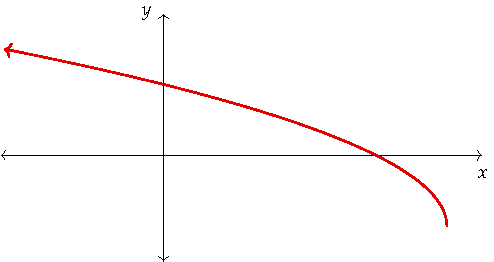
\includegraphics{intercepts1}
\vfill[1]






\example
The graph of the equation
$y=2+ \dfrac{1}{1-x}$
is given below.
Find the $x$-intercept and the $y$-intercept of the graph.

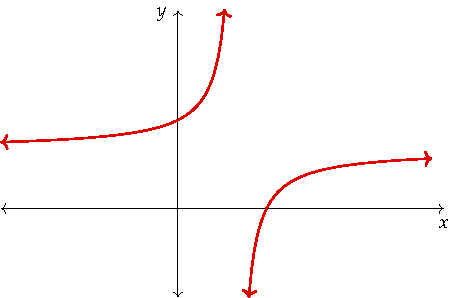
\includegraphics{intercepts2}
\vfill


\newpage



\example
Find the $x$-intercept and the $y$-intercept of the graph of
$2x-3y=6$.
Use the intercepts to graph the equation.

\cart{6}
\vfill


%\example
%The local pet shop charges $12$\textcent \, per cricket up to 100 crickets, and $10$\textcent \, per cricket thereafter.  Write a piecewise-defined linear function which calculates the price $P$, in dollars, of purchasing $c$ crickets.





\begin{goals}
I know how to graph the library of functions.  \\
I know the domain and range for the library of functions. \\
I know how to find the $x$ and $y$-intercept of a graph. \\
I know how to construct a piecewise function. \\
I know how to evaluate values for a piecewise function. \\
I know how to graph a piecewise function. \\
\end{goals}




\end{document}
